\section{Trabalhos Relacionados}
\label{section:trabalhos_relacionados}


Este tópico é destinado a listar uma sequência de trabalhos científicos nas 
áreas abordadas por este estudo com o objetivo de adquirir conhecimento para a
elaboração do mesmo.

Segundo \citeauthoronline{silvio_taynan:2017} (\citeyear{silvio_taynan:2017}), 
à prova de redação do ENEM é avaliada levando em conta uma matriz de referência 
do \citeauthor{edital_enem:2016} (\citeyear{edital_enem:2016}). Essa matriz, 
foi desenvolvida com a colaboração de especialistas, com o objetivo de 
operacionalizar o exame. A matriz apresenta cinco competências, para cada 
competência expressa para redação existem níveis de conhecimento associados de 
0 a 5. \citeauthoronline{braga:2015} (\citeyear{braga:2015}) explica em seu 
trabalho, que em um texto de redação, o candidato defenderá uma opinião a 
respeito do tema proposto, de forma coerente e coesa, embasado em argumentos 
consistentes. O texto será redigido respeitando a escrita formal da Língua 
Portuguesa. Ao fim, o candidato elabora uma proposta de intervenção social para 
o problema apresentado no desenvolvimento do texto que respeite os direitos 
humanos.

% \begin{longtable}{|c|l|l|}
%     \caption{Competência I de V da matriz de referência elaborada pelo
%     \cite{matriz_referencia_redacao:2016}.}
%     \label{table:matriz_referencia}
%     \endfirsthead
%     \hline
%     \multirow{7}{*}{\textbf{I}} & \multicolumn{2}{l|}{\textbf{Demonstrar domínio da norma padrão da língua escrita.}} \\ \cline{2-3} 
%      & 0 & \begin{tabular}[c]{@{}l@{}}Demonstra desconhecimento da modalidade escrita formal da \\ língua portuguesa.\end{tabular} \\ \cline{2-3} 
%      & 1 & \begin{tabular}[c]{@{}l@{}}Demonstra domínio precário da modalidade escrita formal da \\ língua portuguesa, de forma sistemática, com diversificados e \\ frequentes desvios gramaticais, de escolha de registro e de \\ convenções da escrita.\end{tabular} \\ \cline{2-3} 
%      & 2 & \begin{tabular}[c]{@{}l@{}}Demonstra domínio insuficiente da modalidade escrita formal \\ da língua portuguesa, com muitos desvios gramaticais, de \\ escolha de registro e de convenções da escrita.\end{tabular} \\ \cline{2-3} 
%      & 3 & \begin{tabular}[c]{@{}l@{}}Demonstra domínio mediano da modalidade escrita formal da \\ língua portuguesa e de escolha de registro, com alguns desvios \\ gramaticais e de convenções da escrita.\end{tabular} \\ \cline{2-3} 
%      & 4 & \begin{tabular}[c]{@{}l@{}}Demonstra bom domínio da modalidade escrita formal da língua \\ portuguesa e de escolha de registro,com poucos desvios \\ gramaticais e de convenções da escrita.\end{tabular} \\ \cline{2-3} 
%      & 5 & \begin{tabular}[c]{@{}l@{}}Demonstra excelente domínio da modalidade escrita formal da \\ língua portuguesa e de escolha de registro. Desvios gramaticais \\ ou de convenções da escrita serão aceitos somente como \\ excepcionalidade e quando não caracterizem reincidência.\end{tabular} \\ \hline
    % \multirow{7}{*}{\textbf{II}} & \multicolumn{2}{l|}{\textbf{\begin{tabular}[c]{@{}l@{}}Compreender a proposta de redação e aplicar conceitos \\ das varias áreas de conhecimento para desenvolver o tema, \\ dentro dos limites estruturais do texto \\ dissertativo-argumentativo em prosa.\end{tabular}}} \\ \cline{2-3} 
    %  & 0 & \begin{tabular}[c]{@{}l@{}}``Fuga ao tema/não atendimento à estrutura \\ dissertativo-argumentativa''.\end{tabular} \\ \cline{2-3} 
    %  & 1 & \begin{tabular}[c]{@{}l@{}}Apresenta o assunto, tangenciando o tema ou demonstra \\ domínio precário do texto dissertativo-argumentativo, com \\ traços constantes de outros tipos textuais\end{tabular} \\ \cline{2-3} 
    %  & 2 & \begin{tabular}[c]{@{}l@{}}Desenvolve o tema recorrendo à cópia de trechos dos textos \\ motivadores ou apresenta domínio insuficiente do texto \\ dissertativo-argumentativo, não atendendo à estrutura com \\ proposição, argumentação e conclusão.\end{tabular} \\ \cline{2-3} 
    %  & 3 & \begin{tabular}[c]{@{}l@{}}Desenvolve o tema por meio de argumentação previsível e \\ apresenta domínio mediano do texto dissertativo-argumentativo, \\ com proposição, argumentação e conclusão.\end{tabular} \\ \cline{2-3} 
    %  & 4 & \begin{tabular}[c]{@{}l@{}}Desenvolve o tema por meio de argumentação consistente e \\ apresenta bom domínio do texto dissertativo-argumentativo, \\ com proposição, argumentação e conclusão.\end{tabular} \\ \cline{2-3} 
    %  & 5 & \begin{tabular}[c]{@{}l@{}}Desenvolve o tema por meio de argumentação consistente, a \\ partir de um repertório sócio cultural produtivo e apresenta \\ excelente domínio do texto dissertativo-argumentativo.\end{tabular} \\ \hline
    % \multirow{7}{*}{\textbf{III}} & \multicolumn{2}{l|}{\textbf{\begin{tabular}[c]{@{}l@{}}Selecionar, relacionar, organizar e interpretar informações, \\ fatos, opiniões e argumentos em defesa de um ponto de vista.\end{tabular}}} \\ \cline{2-3} 
    %  & 0 & \begin{tabular}[c]{@{}l@{}}Apresenta informações, fatos e opiniões não relacionados \\ ao tema e sem defesa de um ponto de vista.\end{tabular} \\ \cline{2-3} 
    %  & 1 & \begin{tabular}[c]{@{}l@{}}Apresenta informações, fatos e opiniões pouco relacionados \\ ao tema ou incoerentes e sem defesa de um ponto de vista.\end{tabular} \\ \cline{2-3} 
    %  & 2 & \begin{tabular}[c]{@{}l@{}}Apresenta informações, fatos e opiniões relacionados ao \\ tema, mas desorganizados ou contraditórios e limitados aos \\ argumentos dos textos motivadores, em defesa de um \\ ponto de vista.\end{tabular} \\ \cline{2-3} 
    %  & 3 & \begin{tabular}[c]{@{}l@{}}Apresenta informações, fatos e opiniões relacionados ao tema, \\ limitados aos argumentos dos textos motivadores e pouco \\ organizados, em defesa de um ponto de vista.\end{tabular} \\ \cline{2-3} 
    %  & 4 & \begin{tabular}[c]{@{}l@{}}Apresenta informações, fatos e opiniões relacionados ao tema, \\ de forma organizada, com indícios de autoria, em defesa de \\ um ponto de vista.\end{tabular} \\ \cline{2-3} 
    %  & 5 & \begin{tabular}[c]{@{}l@{}}Apresenta informações, fatos e opiniões relacionados ao \\ tema proposto, de forma consistente e organizada, configurando \\ autoria, em defesa de um ponto de vista.\end{tabular} \\ \hline
    % \multirow{7}{*}{\textbf{IV}} & \multicolumn{2}{l|}{\textbf{\begin{tabular}[c]{@{}l@{}}Demonstrar conhecimento dos mecanismos linguísticos \\ necessários para a construção da argumentação.\end{tabular}}} \\ \cline{2-3} 
    %  & 0 & Não articula as informações. \\ \cline{2-3} 
    %  & 1 & Articula as partes do texto de forma precária. \\ \cline{2-3} 
    %  & 2 & \begin{tabular}[c]{@{}l@{}}Articula as partes do texto, de forma insuficiente, com muitas \\ inadequações e apresenta repertório limitado de recursos coesivos.\end{tabular} \\ \cline{2-3} 
    %  & 3 & \begin{tabular}[c]{@{}l@{}}Articula as partes do texto, de forma mediana, com inadequações, \\ e apresenta repertório pouco diversificado de recursos coesivos.\end{tabular} \\ \cline{2-3} 
    %  & 4 & \begin{tabular}[c]{@{}l@{}}Articula as partes do texto com poucas inadequações e apresenta \\ repertório diversificado de recursos coesivos.\end{tabular} \\ \cline{2-3} 
    %  & 5 & \begin{tabular}[c]{@{}l@{}}Articula bem as partes do texto e apresenta repertório diversificado \\ de recursos coesivos.\end{tabular} \\ \hline
    % \multirow{7}{*}{\textbf{V}} & \multicolumn{2}{l|}{\textbf{\begin{tabular}[c]{@{}l@{}}Elaborar proposta de intervenção para o problema abordado, \\ respeitando os direitos humanos.\end{tabular}}} \\ \cline{2-3} 
    %  & 0 & \begin{tabular}[c]{@{}l@{}}Não apresenta proposta de intervenção ou apresenta proposta não \\ relacionada ao tema ou ao assunto.\end{tabular} \\ \cline{2-3} 
    %  & 1 & \begin{tabular}[c]{@{}l@{}}Apresenta proposta de intervenção vaga, precária ou relacionada \\ apenas ao assunto.\end{tabular} \\ \cline{2-3} 
    %  & 2 & \begin{tabular}[c]{@{}l@{}}Elabora, de forma insuficiente, proposta de intervenção relacionada \\ ao tema, ou não articulada com adiscussão desenvolvida no texto.\end{tabular} \\ \cline{2-3} 
    %  & 3 & \begin{tabular}[c]{@{}l@{}}Elabora, de forma mediana, proposta de intervenção relacionada ao \\ tema e articulada à discussão desenvolvida no texto.\end{tabular} \\ \cline{2-3} 
    %  & 4 & \begin{tabular}[c]{@{}l@{}}Elabora bem proposta de intervenção relacionada ao tema e \\ articulada à discussão desenvolvida no texto.\end{tabular} \\ \cline{2-3} 
    %  & 5 & \begin{tabular}[c]{@{}l@{}}Elabora muito bem proposta de intervenção, detalhada, relacionada \\ ao tema e articulada à discussão desenvolvida no texto.\end{tabular} \\ \hline
% \end{longtable}

Em seu estudo \citeauthoronline{monard_baranauskas:2003} 
(\citeyear{monard_baranauskas:2003}) cita: ``A indução é a forma de 
inferência lógica que permite obter conclusões genéricas sobre um conjunto 
particular de exemplos.'' Na indução, um conceito é aprendido efetuando-se 
inferência indutiva sobre os exemplos apresentados. O aprendizado indutivo 
pode ser dividido em supervisionado e não-supervisionado como ilustrada a 
Figura \ref{figure:aprendizado_indutivo}. No aprendizado não-supervisionado, o 
algoritmo de aprendizado analisa os exemplos fornecidos e tenta determinar se 
alguns deles podem ser agrupados de alguma maneira, formando \textit{clusters} 
ou agrupamentos. Já no aprendizado supervisionado é fornecido ao algoritmo de 
aprendizado um conjunto de exemplos de treinamento para os quais o rótulo da 
classe associada é conhecido.

\begin{figure}[H]
\begin{center}
    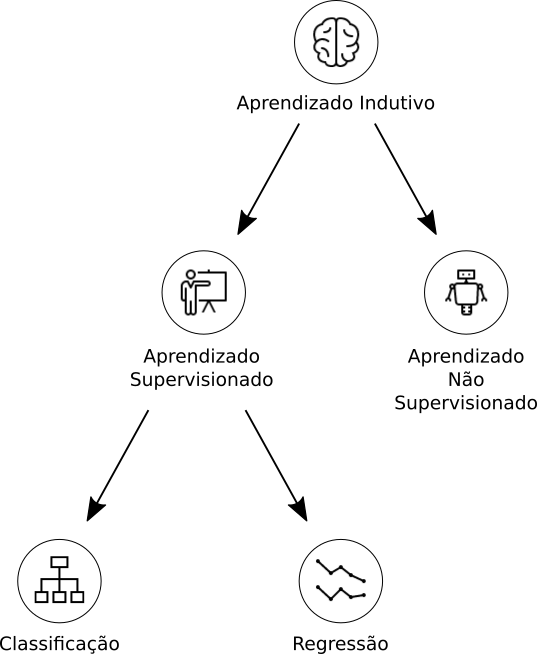
\includegraphics[scale=0.40]{images/aprendizado_indutivo.png}
\end{center}
\caption{Árvore hierárquica do aprendizado indutivo, a qual é dividida em 
algoritmos supervisionado e não-supervisionado.}
\label{figure:aprendizado_indutivo}
\end{figure}

Classificadores são utilizados para a predição de classes de objetos e pode ser 
dita como o processo de generalização dos dados a partir de diferentes 
instâncias. Existe uma tendência de se referir a problemas com uma resposta 
quantitativas como problemas de regressão e aqueles com uma resposta 
qualitativa como problemas de classificação. Dado um conjunto de exemplos como 
ilustrado na Figura \ref{figure:processo_classificacao}, os classificadores 
devem encontrar uma função geral capaz de prever adequadamente as saídas para 
novos exemplos, após o treinamento, o classificador é avaliado e se necessário 
o processo de classificação pode ser ajustado usando o conhecimento sobre o 
domínio do problema para escolher os dados de entrada ao algoritmo de 
aprendizado de acordo com \citeauthoronline{porthos_motta:2016} 
(\citeyear{porthos_motta:2016}).

\begin{figure}[H]
\begin{center}
    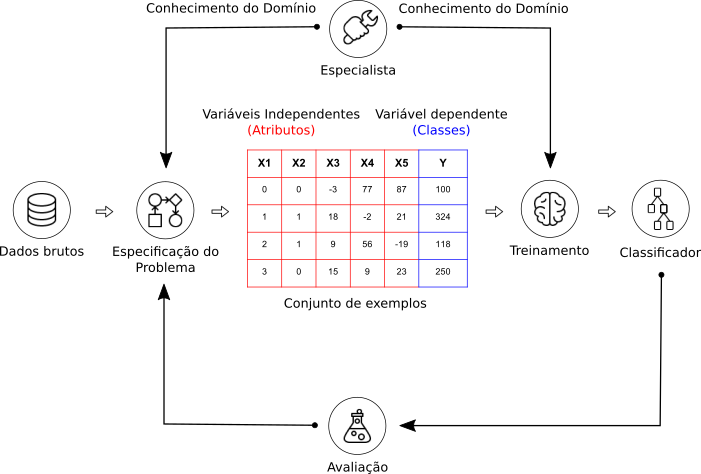
\includegraphics[scale=0.60]{images/processo_classificacao.png}
\end{center}
\caption{Fluxo do processo de classificação, o modelo encontra uma função geral 
capaz de prever as saídas, a especificação do problema pode ser reajustada com 
o conhecimento do domínio para obter um melhor resultado.}
\label{figure:processo_classificacao}
\end{figure}

Diversas ferramentas disponíveis para exploração de dados dispõem de soluções 
para o processamento e a análise das informações de forma ágil e simples. 
Em uma análise comparativa \citeauthoronline{boscarioli2014avaliaccao} 
(\citeyear{boscarioli2014avaliaccao}) demonstra que não 
existe uma única ferramenta com características melhores para todas as 
aplicações em mineração de dados. Em um estudo que comparou quatro ferramentas 
(KMINE, \textit{Orange}, Tanagra, Weka), todas de código aberto, gratuitas e 
muito utilizadas na pesquisa e na academia, \citeauthoronline{wahbeh2011comparison} 
(\citeyear{wahbeh2011comparison}) concluiu que a ferramenta Weka apresentou o 
melhor desempenho, seguido pelo \textit{Orange}, e, depois, pelo KMINE e 
Tanagra. De acordo com \cite{JMLR:demsar13a}, a ferramenta \textit{Orange} na 
atual versão 3.5 desenvolvida pelo laboratório de Inteligência Artificial da 
Faculdade de Computação e Ciência da Informação da Universidade de 
\textit{Ljubljana} na \textit{Eslovênia} sob a licença GPL, possui uma 
interface gráfica denominada \textit{Orange Canvas}. Por meio de sua interface 
gráfica denominada \textit{Orange Canvas}, é possível conectar e interligar os 
objetos montando um fluxo de trabalho para o desenvolvimento de modelos de 
classificação, incluindo \textit{Adaboost}, \textit{Naive Bayes}, Regras de 
Decisão, Árvores de Decisão, etc..

% Por meio de sua interface 
% ilustrada na Figura \ref{figure:orange_canvas} é possível conectar e interligar 
% os objetos montando um fluxo de trabalho para o desenvolvimento de modelos de 
% classificação, incluindo \textit{Adaboost}, \textit{Naive Bayes}, Regras de 
% Decisão, Árvores de Decisão, etc..

% \begin{figure}[H]
% \begin{center}
%     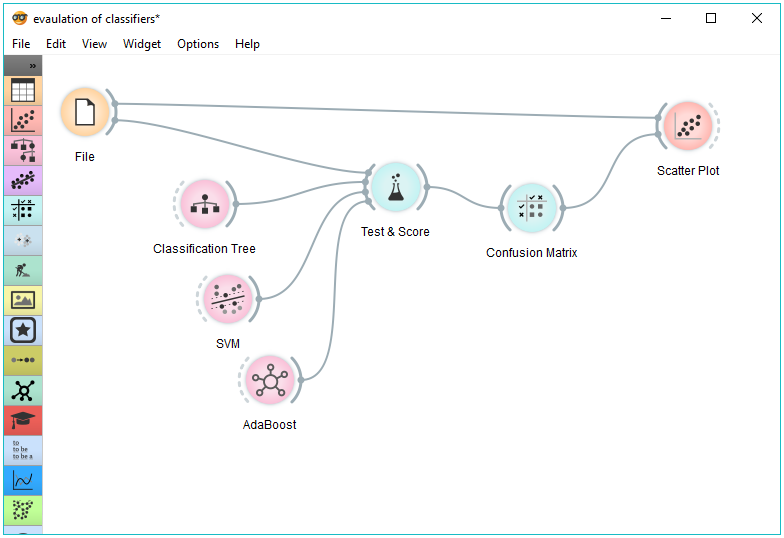
\includegraphics[scale=0.50]{images/orange_canvas.png}
% \end{center}
% \caption{Ferramenta de mineração de dados \textit{Orange Canvas}} 
% executando teste de desempenho dos classificadores AdaBoost, SVM e 
% \textit{Classification Tree} na matriz de confusão.  
% \label{figure:orange_canvas}
% \end{figure}

No processo de mineração de dados, segundo 
\citeauthoronline{matsubara2003pretext} (\citeyear{matsubara2003pretext}) , na 
etapa de pré-processamento de textos, um dos métodos geralmente adotado é a 
representação usando a abordagem ``bag-of-words'', uma das representações 
estruturadas mais simples, que utiliza técnicas de redução do termo ao seu 
radical e remoção de termos irrelevantes. Cada documento é  representado como 
um vetor de palavras que ocorrem no documento, especificamente uma tabela 
atributo-valor. 

Segundo a pesquisa de \citeauthoronline{de2017mineraccao} 
(\citeyear{de2017mineraccao}), o classificador Naive Bayes é um 
progenitor probalístico para textos, está entre um dos mais utilizados no 
Aprendizado de Máquina, devido a seu comportamento simplista que traz bons 
resultados em muitos casos. Baseado no Teorema de Bayes, criado por Thomas 
Bayes no século XVIII, este classificador é eleito o mais eficiente na precisão 
e rotulação de novas amostras de acordo com o trabalho de 
\citeauthoronline{chakrabarti2002mining} (\citeyear{chakrabarti2002mining}). 
Objetivo da classificação Naive Bayes é encontrar a melhor classe, uma 
característica atraente desse classificador.

Um dos algoritmos mais famoso e utilizado no Aprendizado de Máquina é 
\textit{AdaBoost} ou \textit{Adaptive Boosting} derivado do \textit{Boosting}, 
uma técnica de Aprendizado de Máquina que usa diversos classificadores 
fracos com a finalidade de aumentar a acurácia geral. Segundo 
\citeauthoronline{dos2015detecccao} 
(\citeyear{dos2015detecccao}), o seu sucesso deve-se ao merito 
de conseguir adaptar-se aos classificadores base. Neste algoritmo, 
classificadores são gerados de forma a ajudar os exemplos incorretamente 
classificados pelos classificadores antecedentes. Este algoritmo aumenta os 
pesos dos exemplos em que os classificadores anteriores cometeram erros.